\section{Railway network}
The flatland environment is simulated by a rectangular grid of fixed size, which can be set by the user. Each cell of the grid is either a rail cell, or an empty unusable cell, or a \textbf{target} cell. Rails are of different type, depending on the available \textbf{transitions}: there are 16 different transitions in flatland, since there are 4 different orientations, and 4 other directions of exit from the cell. Thus, each cell is described by a bitmap that represents the whole transition space.\\
However, not every transition is allowed in flatland.\ Since the aim is to actually simulate a real railway system, only a maximum of 2 exit directions are allowed from every orientation of the agent, which result in 8 different cell types (including empty ones).\\ \\
Flatland offers also a \textit{sparse\_rail\_generator} that randomizes the creation of a realistic railway structure, where clusters of cities are sparsely connected to each other, allowing to mimic as faithfully as possible real city railway networks.

\begin{figure}[H] 
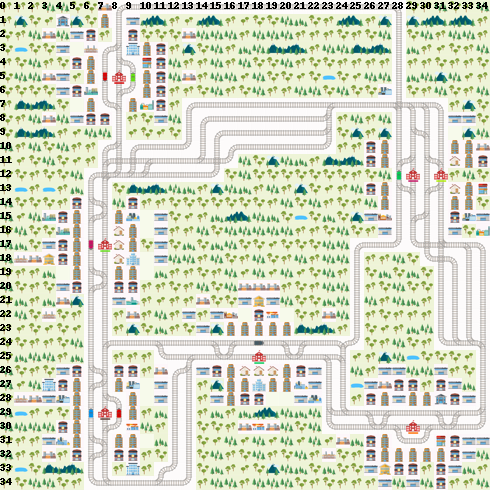
\includegraphics[height=80mm, width=80mm, scale=0.5]{figures/sparse_railway.png}
\centering
\caption{Sparse railway}
\label{fig:s1}
\end{figure}

\section{Agents}
Trains have a number of important properties:
\begin{itemize}
\item \textbf{Position}: the current coordinates of the agent.
\item \textbf{Target}: the position of the target cell.
\item \textbf{Direction}: the current orientation described with an integer\\
    \verb|[0=North, 1=Est, 2=South, 3=West]|
\item \textbf{Movement}: an integer describing the status of the agent\\
    \verb|[0=READY_TO_DEPART, 1=ACTIVE, 2=DONE, 3=DONE_REMOVED]|
\end{itemize}
\noindent
Since every agent is liable to malfunctions, much like real trains, there are properties to keep track of that in addition to variables that store the agents' speed:
\begin{itemize}
\item \textbf{Malfunction rate}: the Poisson rate at which malfunctions occur
\item \textbf{Malfunction}: a counter of the remaining time the agent will remain malfunctioning
\item \textbf{Next malfunction}: number of steps until next malfunction will occour
\item \textbf{Number of malfunctions}: the total number of malfunctions for this agent
\item \textbf{Max speed}: a fraction between 0 and 1. (\textit{e.g.} a speed of 1/2 means that the agent changes cell after 2 time steps)
\item \textbf{Position fraction}: related to speed, indicates when the next action can be taken
\end{itemize}
\section{Environment Actions}
\label{sec:envActions}
The available actions are:
\begin{itemize}
\item \textbf{DO NOTHING (0)}: Default action if None has been provided or the value is not within this list. If agent.moving is True then the agent will \textit{MOVE\_FORWARD}.

\item \textbf{MOVE LEFT (1)}: If the transitions of the current cell allows it, the agent change its direction towards the left, otherwise the action is masked with a \textit{MOVE\_FORWARD}. If the agent is not moving then update also it's state to moving.

\item \textbf{MOVE FORWARD (2)}: It updates the direction of the agent following the transitions allowed in the current cell. If the cell is a dead-end the new direction is the opposite of the current. If the agent is not moving then update also it's state to moving.

\item \textbf{MOVE RIGHT (3)}: If the transitions of the current cell allows it, the agent change it's direction toward the right, otherwise the action is masked with a \textit{MOVE\_FORWARD}. If the agent is not moving then update also its state to moving.

\item \textbf{STOP MOVING (4)}: Stop the agent in the current occupied cell and cause the change of value of the variable describing the state of the agent.

\end{itemize}
\section{Rewards}
\label{sec:envRewards}
The rewards are based on the following values:
\begin{itemize}
\item \textit{invalid action}: penalty which is currently set to 0, penalty for requesting an invalid action
\item \textit{step penalty}: which is -1 * alpha, penalty for a time step.
\item \textit{global reward}: calculated as 1 * beta, a sort of default reward.
\item \textit{stop penalty}: is currently set to 0, penalty for stopping a moving agent
\item \textit{start penalty}: is currently set to 0, penalty for starting a stopped agent
\end{itemize}
The full step penalty is computed as the product between \textit{step penalty} and agent speed data (\textit{i.e.} the \textit{speed} variable).\
There are different rewards for different situations:
\begin{itemize}
\item agents that are in status \textit{DONE} or \textit{DONE\_REMOVED} have zero reward.
\item all agents that have finished in this episode (checked at the end of the step), have reward equal to the global reward (when in step all agents have reached their target)

\item full step penalty is assigned when an agent is in state \textit{READY\_TO\_DEPART} and in the current turn moves or stay there (2th step agent case), or when is in malfunction.
\item full step penalty plus the other penalties (invalid action penalty, stop penalty and start penalty) when the agent is finishing actions or start new ones. Currently the other penalties are all set to zero.
\end{itemize}
Currently it is possible to say that agents’ rewards are always full step, excluding when the episode ends and when they have finished, where is 0.

